% ================================== HEADER ====================================
\documentclass{article}           % Sets style/look of many things.
% \documentclass{report}          % part, chapters, front page etc.
\usepackage{exsheets}
\usepackage[utf8]{inputenc}       % Encoding of input files UTF-8
\usepackage[T1]{fontenc}
\usepackage[scaled]{beramono}     % Font
\usepackage{color}                % Color text
\usepackage{titlesec}             % Select alternative section titles
\usepackage{fancyvrb}
\usepackage{verbatim}             % Comment environment
\usepackage{listings}             % Format and render text/code etc.
\usepackage{minted}               % Much better syntax highlighting
\usepackage{float}                % Control of floating environment/figure
\usepackage{graphicx,  subfigure} % Better figures, graphics, units etc.
\usepackage{multicol}             % Multiple columns
\usepackage{amsmath}              % Math: Equation, split, align etc.
\usepackage{siunitx}              % SI units
\usepackage{mathtools}            % Different math tools to use with amsmath
\usepackage{amssymb}              % Math symbols
\usepackage[
    colorlinks,
    citecolor=black,              % I like links with standard black color
    filecolor=black,
    linkcolor=black,
    urlcolor=black
]{hyperref}                       % Links in TOC etc.
\usepackage[all]{hypcap}          % Better links to floating environment

\usepackage{tabto}
\newcommand\marginsymbol[1][0pt]{%
  \tabto*{0cm}\makebox[\dimexpr-1cm-#1\relax][r]{$\mathbb{P}$}\tabto*{\TabPrevPos}}

\renewcommand{\thesubsection}{\thesection.\alph{subsection}}
\title{\vspace{-2cm}INF3490/INF4490 Exercise Solutions - Week 1}
\author{Ole Herman S. Elgesem}
\date{\today}

% Removing paragraph indents is sometimes useful:
\setlength\parindent{0pt}

% Make margins smaller to fit more figures, tables etc on page: (optional)
\addtolength{\oddsidemargin}{-1.0in}
\addtolength{\evensidemargin}{-1.0in}
\addtolength{\textwidth}{2.0in}
\addtolength{\topmargin}{-0.8in}
\addtolength{\textheight}{1.6in}
% ==============================================================================

% ================================= DOCUMENT ===================================
\begin{document}
    \renewcommand\marginsymbol[1][0pt]{%
  \tabto*{0cm}\makebox[-1cm][c]{$\mathbb{P}$}\tabto*{\TabPrevPos}}

\maketitle
\(\mathbb{P}\) marks the programming exercises, we strongly recommend using
the python programming language for these. Exercises may be added/changed
after publishing.


\section{Simple search algorithms}

Given the function \(f(x) = -x^4 + 2x^3 + 2x^2 - x\):

\subsection{Derivative}
What is its derivative \(f'(x)\) ?\\

\textit{Answer:}
\[f'(x) = -4x^3 + 6x^2 + 4x - 1\]

\subsection{Plotting \marginsymbol}
Plot the function, and its gradient(derivative) from \(x=-2\) to \(x=3\).
Use python, wolfram alpha or another plotting tool of your choice.\\

\emph{Plot:}
\begin{figure}[H]
\begin{center}
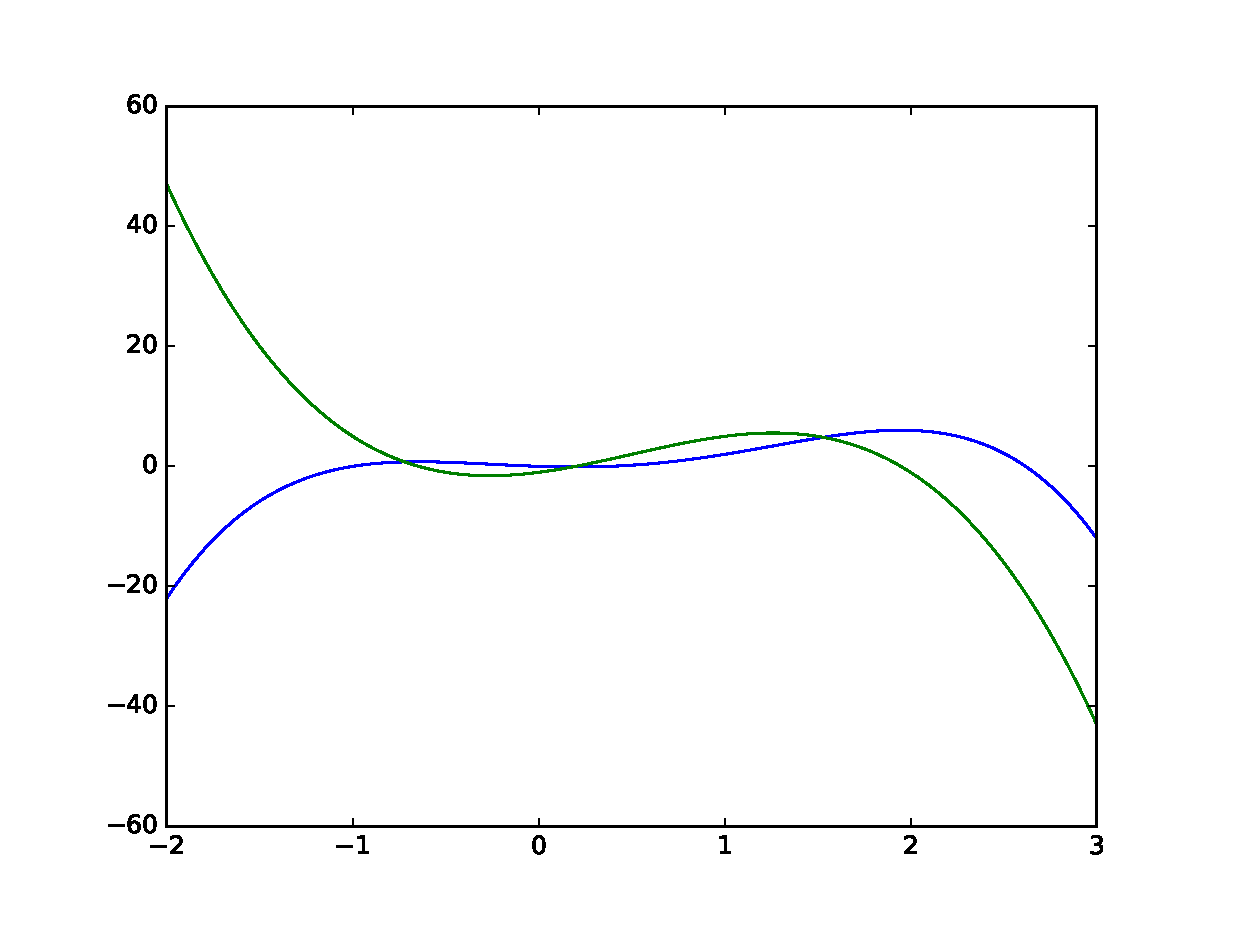
\includegraphics[width=0.6\textwidth]{eps/w1e1b.eps}
\caption{\(f(x)\) and it's derivative.}
\label{fig:w1e1b}
\end{center}
\end{figure}

\emph{Source code (Python 3):}
\inputminted{Python}{py/w1e1b.py}

\subsection{Gradient Ascent \marginsymbol}
\label{subsec:grada}
Maximize using gradient ascent.
You can try step size 0.1 and start somewhere in the range [-2, 3].
How does the choice of starting point and step size affect the algorithm's performance?
Is there a starting point where the algorithm would not even be able to find a local maximum?\\

\textit{Answer:}

Both starting position and step size affects where the algorithm ends:
\begin{itemize}
    \item Starting Position
    \begin{itemize}
        \item \emph{Left side:} Should converge on left maximum
        \item \emph{Center:} Stops immediately, gradient is zero.
        \item \emph{Right side:} Should converge on right maximum
    \end{itemize}
    \item Step Size
    \begin{itemize}
        \item \emph{Too low:} Converges slowly (poor performance)
        \item \emph{Too high:} Overshoot, bounce over solutions. Doesn't converge, might not terminate.
    \end{itemize}
\end{itemize}

\emph{Plot:}
\begin{figure}[H]
\begin{center}
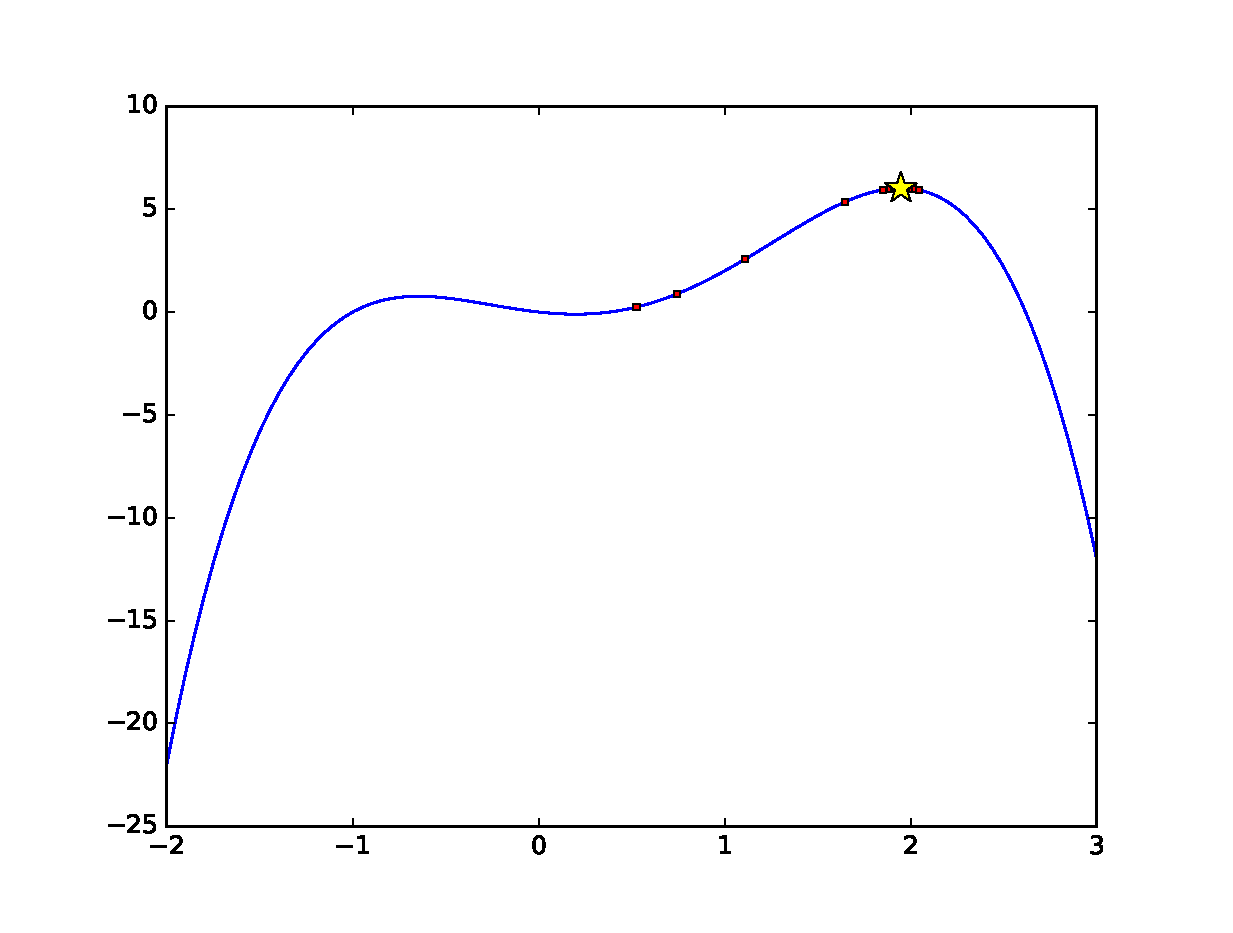
\includegraphics[width=0.6\textwidth]{eps/w1e1c.eps}
\caption{Result of gradient ascent}
\label{fig:w1e1c}
\end{center}
\end{figure}

\emph{Source code (Python 3):}
\inputminted{Python}{py/w1e1c.py}

\subsection{Exhaustive Search \marginsymbol}
\label{subsec:exhaust}
Assume that we are only interested in maxima of \(f(x)\) where
\(-2\leq x \leq 3\), and \(x\) increases in steps of length 0.5.
(\(\Delta x = 0.5\)). Perform an exhaustive search to
maximize \(f(x)\) and plot the result.\\

\emph{Plot:}
\begin{figure}[H]
\begin{center}
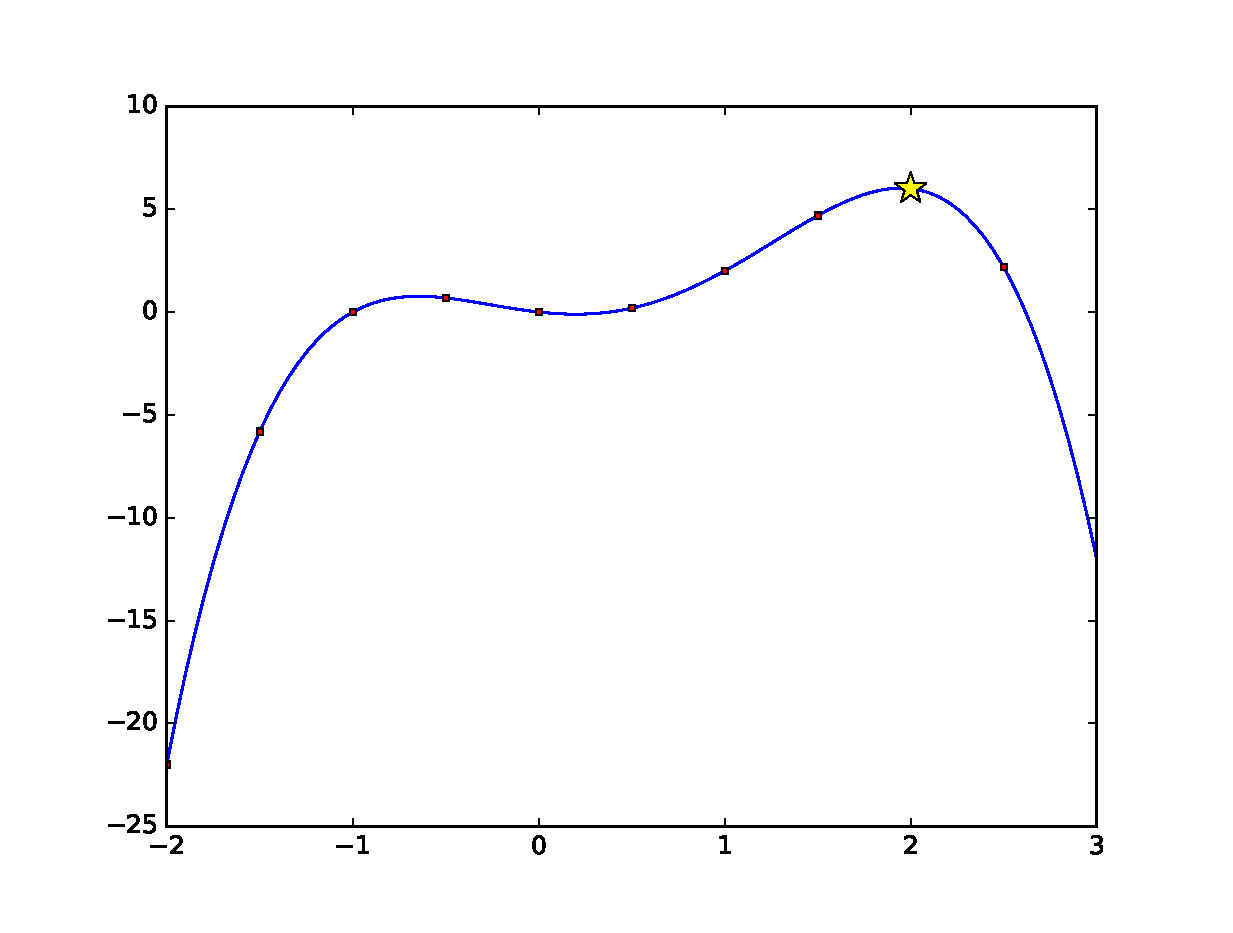
\includegraphics[width=0.6\textwidth]{eps/w1e1d.eps}
\caption{Result of exhaustive search}
\label{fig:w1e1c}
\end{center}
\end{figure}

\emph{Source code (Python 3):}
\inputminted{Python}{py/w1e1d.py}

\subsection{Greedy Search and Hill Climbing}
In what way would greedy search and hill climbing differ for the maximization problem in Problem \ref{subsec:grada}?
Can you identify a starting position where the two algorithms might give different results?\\

\textit{Answer:}

Greedy search will check all neighbors and always go in most promising direction.
Hill climber will randomly find a decent neighbor and walk there.
If both algorithms started in center ( \(x = 0.5\) ),
greedy search always go right,
while hill climber could go right and left ( 50/50 ) as both are \emph{up}.

\subsection{Possible improvements}
Gradient ascent, greedy search and hill climbing are quite similar,
and are all based almost exclusively on exploitation.
Can you think of any additions to these algorithms in order to do more exploration?\\

\textit{Answer:}

Run the algorithm several times with random starting positions,
this will \emph{explore} the solution space and find several local optima.
Another option is to add more random movement to either algorithm.
This can be done after a solution is found, or at a probability while searching.
Could also do backtrack + random jump after a solution is found.

\subsection{Exhaustive search vs. simulated annealing}
Which algorithm do you think is the most efficient at maximizing \(f(x)\) under the conditions in Problem \ref{subsec:exhaust}: exhaustive search or simulated annealing?
Explain.\\

\textit{Answer:}

Exhaustive search is better for this case.
It takes few iterations to go through the one dimensional solution space.
For problems in higher dimensions or more complex functions with smaller step size exhaustive search becomes impractical and simulated annealing will outperform.

\section*{Contact and Github}
Corrections of grammar, language, notation or suggestions for improving this material are appreciated.
E-mail me at \href{mailto:olehelg@uio.no}{\textbf{olehelg@uio.no}} or use \href{https://github.com/olehermanse/INF3490-AI_Machine_Learning}{\textbf{GitHub}} to submit an issue or create a pull request.
The \href{https://github.com/olehermanse/INF3490-AI_Machine_Learning}{\textbf{GitHub repository}} contains all source code for assignments, exercises, solutions, examples etc.
As many people have been involved with writing and updating the course material, they are not all listed as authors here.
For a more complete list of authors and contributors see the \href{https://github.com/olehermanse/INF3490-AI_Machine_Learning/blob/master/README.md}{\textbf{README}}.

\end{document}
% ==============================================================================
